\chapter{总结和未来工作}

\section{总结}
随着大数据,云计算和机器视觉的发展,机器视觉的实际应用需要涉及基础设施,云计算,分布式存储,分布式编程,集群部署与管理。
本论文介绍了CloudVision云平台,让研究员只关注机器视觉算法部分,由平台保证高效可靠地执行
大规模数据的机器视觉应用。本论文工作主要分成三部分:
\begin{enumerate}
  \item 各个领域的研究与架构设计(20\%)

        因为CloudVision依赖多个领域,我首先研究每个领域的主流和最佳的方法。基于这个
        研究背景,推出了CloudVision的横向扩展,高可用,高性能的架构。
        在架构考虑到大规模存储,弹性处理和易用性,使用了Spark的分布式处理框架和云平台的
        对象存储,为了提高读写性能采用了Alluxio的分布式内存缓存。

  \item 建立学院的OpenStack私有云(30\%)

        为了CloudVision的实验和学院的需求,建立了清华软件学院的信息系统与工程研究所OpenStack私有云。
        在Cloudvision开发和实验部分,使用了我部署的OpenStack私有云环境。另外,
        我部署的环境提供研究所的同学和老师实际使用:实验室同学使用执行实验;助教和老师
        给做大作业的学生提供服务器环境,大作业结束了收回所有资源。
        
        建立了OpenStack私有云包括的工作有:硬件配置,交换机配置,网络设计,布网线,部署和配置OpenStack
        集群等等。使用了Fuel部署工具部署整个OpenStack平台,总共有8台物理服务器,总体
        大概能创建100到200个虚拟机。
  \item CloudVision云平台的开发,测试和实验(50\%)

        主要开发了三部分:控制管理层,自动部署,机器视觉库。
        控制管理层提供对外API服务和Web界面,由于它集成OpenStack和AWS的云平台建立
        ,部署,配置和管理CloudVision的处理集群。用户可以通过控制层提交机器视觉的
        任务,并且执行在被管理的CloudVision处理集群。

        为了能够让平台易于重复部署,我开发了完全自动化的部署流程。我写了Ansible的roles,
        描述集群里的软件如何安装和配置,主要开发的Ansible roles包括:Mesos, Spark, OpenCV。

        为了证明CloudVision平台的架构,开发了基于Spark和大数据结构的机器视觉库,
        实现SIFT特征抽取,BoW图像表示,分类器。在机器视觉库我做了两个实验:横向扩展性实验和内存缓存实验。
        通过增加计算节点的实验了解到平台的横向扩展性。

\end{enumerate}

\begin{wrapfigure}{r}{0.50\textwidth}
  \centering
    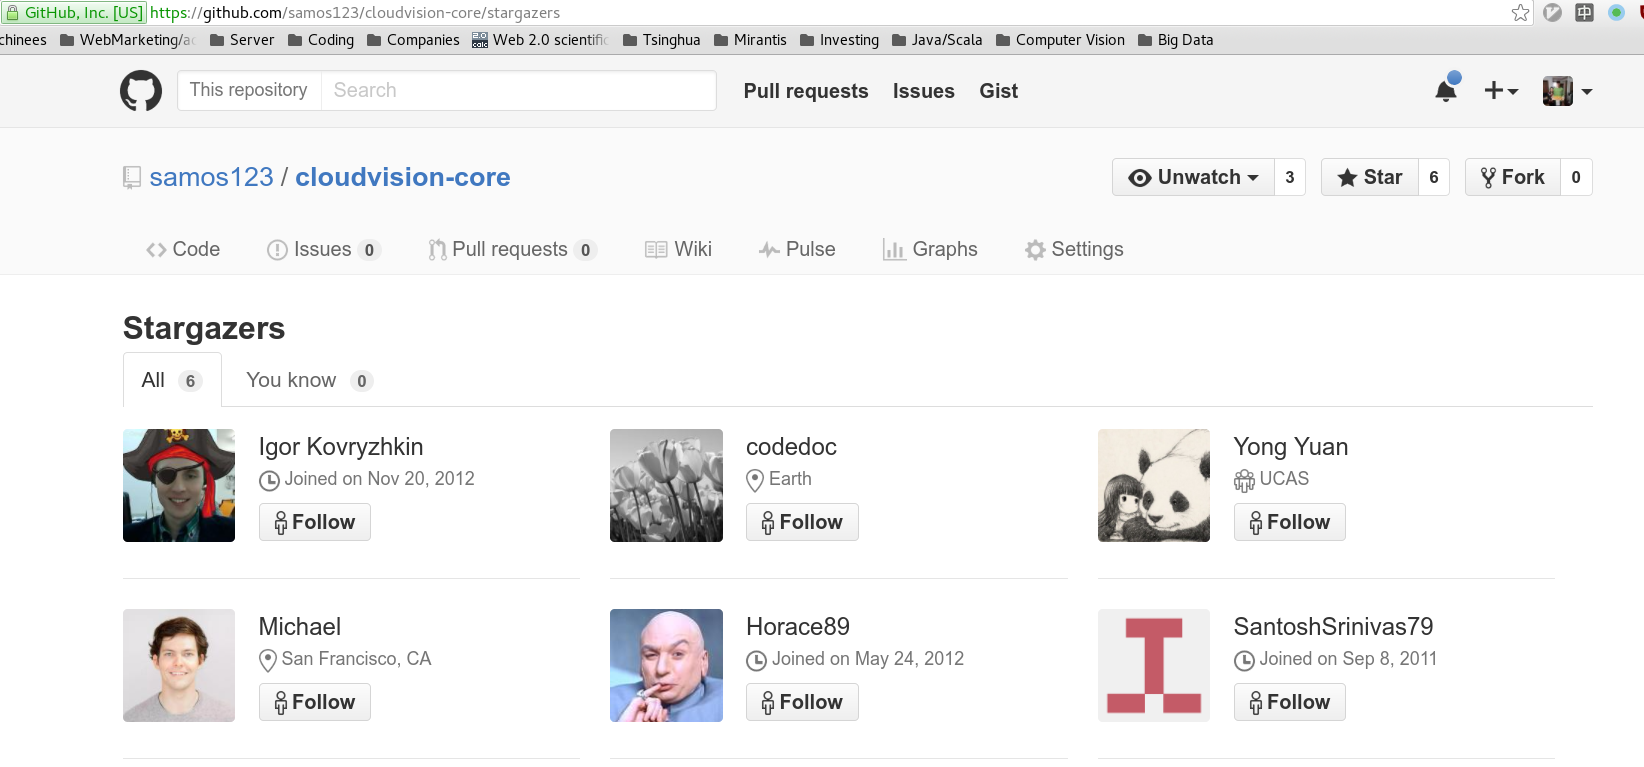
\includegraphics[width=0.49\textwidth]{cloudvision-github-stars}
    \caption{CloudVision在GitHub获得的认可}
  \label{fig:cloudvision-github-stars}
\end{wrapfigure}
我认为CloudVision把机器视觉的PaaS平台基础搭建好了。
在GitHub的开源软件社交网站CloudVision获得了一些认可,在图\ref{fig:cloudvision-github-stars}
可以看到GitHub里有6个用户已经点赞了,包括一个Stanford大学的研究生mdangelo。
虽然基础搭建好了但是还是得提高Spark稳定性和
集成机器视觉最近主流的深度学习。
在稳定性上,发现在Spark执行一些数据量很大的任务,经常会有Out of Memory错误,
然后直接内核杀掉进程。


\section{未来工作}
大部分软件永远完成不了,CloudVision也是这样的软件。其基础部分已经完成,但是为了跟进技术和行业的发展
CloudVision也得不停的更新。我打算以开源的模式继续开发和维护CloudVision平台,未来
打算的工作包括:
\begin{itemize}
  \item 解决Spark稳定性问题

        在实验的时候,我们发现Spark如果长期执行大量数据的任务会发生Out of Memory异常。
        我认为这可能是一个上游的Spark Bug,调研以后发现确实有个Spark bug。\cite{spark-oom-bug}
        Spark还没发布的2.0也会集成Tungsten,Tungsten也能解决多数的Out of Memory异常。
        未来工作包括解决以及升级CloudVision用的Spark版本,同时改进机器视觉库,使用Spark新的
        DataFrame的功能避免依赖PySpark。

  \item 集成深度学习软件

        最近深度学习达到了机器视觉多种应用最好的结果,CloudVision也需要提供
        深度学习的功能,目前有几个主流的软件,Caffe,TensorFlow,SparkNet,Deeplearning4j。
        需要调研哪个软件会变成未来的趋势,支持大规模分布式训练。前期调研认为Google开发的
        TensorFlow会变成深度学习的标准。我打算集成TensorFlow到CloudVision里面,让用户
        通过CloudVision部署和管理TensorFlow集群,同时通过CloudVision提交TensorFlow的任务。

  \item 集成AWS和其他公有云

        CloudVision的架构和实现抽象了云平台的资源,但是目前只有集成和测试基于OpenStack API的
        云平台。未来也可以同样集成其他云平台,比如AWS,Azure,Google Cloud等等。

\end{itemize}



